\documentclass[10pt,a4paper,twocolumn]{article}

\usepackage[a4paper,top=0.75in,bottom=1.18in,left=0.51in,right=0.51in,columnsep=0.25in]{geometry}
\usepackage[T1]{fontenc}
\usepackage[utf8]{inputenc}
\usepackage{microtype}
\usepackage{mathtools}
\usepackage{amsthm}
\usepackage{newtxtext,newtxmath}
\usepackage{booktabs,multirow,array,tabularx}
\usepackage{graphicx}
\usepackage{tikz}
\usetikzlibrary{arrows.meta,positioning,fit,calc,shapes.geometric,backgrounds,matrix,decorations.pathreplacing}
\usepackage{algorithm}
\usepackage{algpseudocode}
\usepackage{caption}
\usepackage{subcaption}
\usepackage{enumitem}
\usepackage{cite}
\usepackage{xurl}
\usepackage[hidelinks]{hyperref}
\hypersetup{
  pdftitle={Recursive Multi Agent Tiny Recursive Models for Efficient Latent Space Reasoning},
  pdfauthor={Panashe Chiurunge},
  pdfsubject={Recursive multi-agent tiny recursive models and latent-space reasoning},
  pdfkeywords={adaptive computation, agent specialization, latent communication, recursive reasoning, sparse routing, tiny models}
}
\usepackage{fancyhdr}
\usepackage{balance}
\usepackage{siunitx}
\usepackage{pifont}
\usepackage{xcolor}

\definecolor{algred}{RGB}{171,19,30}
\definecolor{softred}{RGB}{249,232,234}
\definecolor{softblue}{RGB}{231,240,250}
\definecolor{softgreen}{RGB}{231,246,237}
\definecolor{softgold}{RGB}{250,244,222}
\definecolor{softgray}{RGB}{242,242,242}
\definecolor{darkgray}{RGB}{55,55,55}

\captionsetup{font=small,labelfont=bf,labelsep=period}
\setlength{\textfloatsep}{7pt plus 2pt minus 2pt}
\setlength{\floatsep}{6pt plus 2pt minus 2pt}
\setlength{\intextsep}{6pt plus 2pt minus 2pt}
\setlength{\abovedisplayskip}{5pt plus 2pt minus 2pt}
\setlength{\belowdisplayskip}{5pt plus 2pt minus 2pt}
\setlength{\parindent}{1em}
\setlength{\parskip}{0pt}
\setlist{nosep,leftmargin=*}

\pagestyle{fancy}
\fancyhf{}
\fancyhead[L]{\footnotesize\sffamily\textbf{ALGORITHMICA}}
\fancyhead[R]{\footnotesize\itshape Algorithmica: International Journal of Computational Sciences}
\fancyfoot[L]{\footnotesize\itshape http://africau.edu/\\All rights reserved}
\fancyfoot[R]{\thepage}
\renewcommand{\headrulewidth}{0pt}
\renewcommand{\footrulewidth}{0pt}
\setlength{\headheight}{15pt}

\newtheorem{definition}{Definition}
\newtheorem{proposition}{Proposition}
\newtheorem{remark}{Remark}
\newtheorem{assumption}{Assumption}
\newtheorem{corollary}{Corollary}

\newcommand{\R}{\mathbb{R}}
\newcommand{\KL}{\operatorname{KL}}
\newcommand{\JSD}{\operatorname{JSD}}
\newcommand{\softmax}{\operatorname{softmax}}
\newcommand{\sigmoid}{\operatorname{sigmoid}}
\newcommand{\TopK}{\operatorname{TopK}}
\newcommand{\Pool}{\operatorname{Pool}}
\newcommand{\LN}{\operatorname{LN}}
\newcommand{\CE}{\operatorname{CE}}
\newcommand{\BCE}{\operatorname{BCE}}
\newcommand{\stopgrad}{\operatorname{sg}}
\newcommand{\Ind}{\mathbb{I}}
\newcommand{\MA}{\textsc{MA-TRM}}
\newcommand{\MALite}{\textsc{MA-TRM-Lite}}

\tikzset{
  block/.style={draw,rounded corners=2pt,minimum height=7mm,minimum width=18mm,align=center,font=\scriptsize,thick},
  smallblock/.style={draw,rounded corners=2pt,minimum height=5.5mm,minimum width=14mm,align=center,font=\scriptsize},
  state/.style={draw,ellipse,minimum height=6mm,minimum width=13mm,align=center,font=\scriptsize},
  arrow/.style={-{Latex[length=2mm]},thick},
  latent/.style={-{Latex[length=2mm]},thick,dashed,algred},
  feedback/.style={-{Latex[length=2mm]},thick,dotted,darkgray},
  group/.style={draw,dashed,rounded corners=3pt,inner sep=4pt}
}

\begin{document}

\twocolumn[
\begin{@twocolumnfalse}
\noindent\begin{minipage}{0.48\textwidth}
\footnotesize\itshape Volume 1, Issue 1, pp. xx-xx, 2026.
\end{minipage}\hfill
\begin{minipage}{0.48\textwidth}\raggedleft
\footnotesize\itshape ISSN (Online): 3106-1435
\end{minipage}

\vspace{0.20in}
{\centering
{\fontsize{24}{27}\selectfont Recursive Multi Agent Tiny Recursive Models for Efficient Latent Space Reasoning\par}
\vspace{0.14in}
{\fontsize{14}{16}\selectfont Panashe Chiurunge\par}
\vspace{0.04in}
{\fontsize{10}{12}\selectfont Deep Analytics, Harare, Zimbabwe\par}
{\fontsize{10}{12}\selectfont Corresponding author email to be inserted\par}
}
\vspace{0.14in}

\noindent\textbf{Abstract: }Tiny recursive models show that a compact network can solve difficult structured reasoning tasks by repeatedly refining a latent state and a candidate answer. Their homogeneous recursion, however, applies the same transformation at every reasoning step, provides limited mechanisms for functional specialization, and may spend equal computation on easy and difficult instances. This paper proposes a recursive multi agent tiny recursive model in which several tiny specialized reasoners collaborate through continuous latent representations. The framework replaces a single recursive network with role conditioned agents, introduces private agent states and a shared workspace, uses residual latent links for communication, and allocates additional recursion when agent predictions disagree. Sparse routing activates only the agents required by the current state, while cell level recursive attention concentrates updates on uncertain output locations. Four collaboration topologies are formalized, namely sequential, mixture, deliberation, and distillation. An inner outer optimization procedure assigns local role competence and global system credit. A composite objective balances answer accuracy, iterative improvement, verification, specialization, consensus, routing balance, computation, and halting. The recommended MA TRM Lite architecture preserves a shared two layer backbone and adds low rank role adapters, lightweight latent links, a verifier, and a dynamic router. We derive parameter and computation bounds, present sufficient conditions for stable recursion, provide executable algorithms, and define a rigorous evaluation protocol for Sudoku, maze, and abstraction reasoning benchmarks. The resulting framework is a testable research proposal and does not claim empirical superiority before controlled parameter matched and compute matched evaluation.

\vspace{0.05in}
\noindent\textbf{Keywords: }adaptive computation: agent specialization: latent communication: multi agent reasoning: recursive neural networks: sparse routing: tiny models
\vspace{0.12in}
\end{@twocolumnfalse}
]

\section{Introduction}
Large language models have made substantial progress on reasoning, but their computational cost and dependence on explicit token generation motivate alternative architectures for compact, task specific reasoning. The Abstraction and Reasoning Corpus, Sudoku, and path finding tasks expose a useful regime in which the required output is structured, exact, and often small relative to the internal computation needed to infer it \cite{chollet2019arc}. Hierarchical Reasoning Models introduced recurrent computation at multiple temporal scales \cite{wang2025hrm}. Tiny Recursive Models, abbreviated TRM, simplified this direction to a single small network that repeatedly updates a latent state and a candidate answer \cite{jolicoeur2025trm}. The published TRM results demonstrate that repeated computation can be a scaling axis distinct from parameter count.

TRM also raises a structural question. If one tiny transformation is useful when applied repeatedly, can a small collection of complementary transformations provide a stronger recursion operator without losing parameter efficiency? Recursive Multi-Agent Systems answer a related question for heterogeneous language model agents by connecting their hidden states through trainable RecursiveLink modules and optimizing the resulting collaboration loop as one differentiable system \cite{yang2026recursivemas}. The present work transfers the underlying principle from billion parameter language agents to tiny non-autoregressive reasoners.

We propose the Recursive Multi-Agent Tiny Recursive Model, abbreviated \MA. Several tiny specialized agents collaboratively refine a shared solution in latent space. The proposed model is designed around eleven principles:
\begin{enumerate}[label=\arabic*)]
\item replace the single recursive network with specialized tiny agents;
\item communicate through latent states rather than decoded intermediate answers;
\item maintain private agent states alongside a shared workspace;
\item use disagreement to allocate recursion;
\item route computation sparsely and dynamically;
\item support sequential, mixture, deliberation, and distillation topologies;
\item train through inner and outer co-optimization;
\item optimize a multi-term system objective;
\item focus recursion on uncertain cells;
\item preserve parameter efficiency through controlled sharing;
\item instantiate these ideas in \MALite.
\end{enumerate}

The paper is architectural and methodological. It defines a falsifiable model family and an evaluation protocol. It deliberately avoids reporting synthetic results or implying empirical gains that have not been measured. This distinction is important because analyses of TRM on ARC suggest that augmentation, task identity conditioning, and test-time voting can materially influence reported accuracy \cite{royeazar2025trmanalysis}. Any credible evaluation of \MA{} must therefore isolate architectural gains from parameter count, compute, augmentation, and identity features.

The principal contributions are as follows. First, we formulate a multi-agent recursive state space with role specialization, private memory, and a shared latent workspace. Second, we define low rank latent links, sparse routing, disagreement-driven halting, and cell-level attention in a common differentiable framework. Third, we formalize four collaboration topologies and a two-stage co-optimization algorithm. Fourth, we provide parameter, runtime, and stability analyses. Fifth, we specify \MALite{} as the recommended first implementation and define a complete benchmark plan.

\section{Background and Motivation}
\subsection{Tiny Recursive Models}
Let an input instance be $x$, the candidate discrete answer at supervision step $t$ be $\hat y_t$, its embedding be $y_t$, and the latent reasoning state be $z_t$. A simplified TRM update applies the same tiny network repeatedly:
\begin{align}
z_{t,j+1} &= f_{\theta}(x,y_t,z_{t,j}), \quad j=0,\ldots,n-1, \label{eq:trm_latent}\\
y_{t+1} &= f_{\theta}(y_t,z_{t,n}), \label{eq:trm_answer}
\end{align}
where $n$ is the number of latent updates inside a deep recursion step. Several deep recursion steps may be executed before the answer head and supervision loss are applied. The released TRM configuration uses a two-layer tiny network and reports strong results with a core network of approximately seven million parameters \cite{jolicoeur2025trm}. The architecture is non-autoregressive, which makes it computationally attractive for structured outputs.

The central advantage of (\ref{eq:trm_latent}) and (\ref{eq:trm_answer}) is parameter reuse. Effective depth grows with the number of recursive evaluations, while the number of learned transformation parameters remains fixed. Its central restriction is homogeneous recursion. The same operator must generate hypotheses, perform transformations, detect errors, and determine completion.

A further concern is that recursive depth does not automatically imply effective iterative reasoning. An independent analysis found that a substantial part of ARC performance can depend on test-time voting and task identity conditioning, and that accuracy may saturate after a small number of recursion steps \cite{royeazar2025trmanalysis}. Probabilistic TRM addresses deterministic convergence by injecting noise into recursive trajectories and selecting among candidates with the existing quality head \cite{sghaier2026ptrm}. These findings motivate explicit diversity, disagreement, and adaptive computation within the recursive model itself.

\subsection{Recursive Multi-Agent Systems}
RecursiveMAS models a multi-agent system as a latent recursion loop. Each agent generates latent thoughts, an inner link maps the agent's last-layer states back into its input embedding space, and an outer link transfers states across heterogeneous agents \cite{yang2026recursivemas}. A residual link has the form
\begin{equation}
R(h)=Ph+W_2\sigma(W_1h), \label{eq:recursive_link_origin}
\end{equation}
where $P$ is either the identity or a dimension-matching projection. The approach supports four collaboration patterns and uses an inner stage to align latent generation, followed by an outer stage that optimizes the complete recursive system.

The proposed \MA{} differs in four important respects. First, the agents are tiny non-autoregressive reasoners, rather than independent language models. Second, the answer is a structured tensor, such as a grid or sequence, rather than text. Third, all agents can share a backbone and differ through low rank role adapters. Fourth, disagreement is used as a direct control signal for routing, spatial attention, and recursion depth.

\subsection{Research Gap}
TRM demonstrates homogeneous recursive reuse, and RecursiveMAS demonstrates latent collaboration among heterogeneous language agents. Neither directly studies the regime in which multiple tiny specialists share most parameters, preserve private states, communicate continuously, route sparsely, and refine a structured answer at cell resolution. \MA{} targets this gap.

\begin{figure*}[t]
\centering
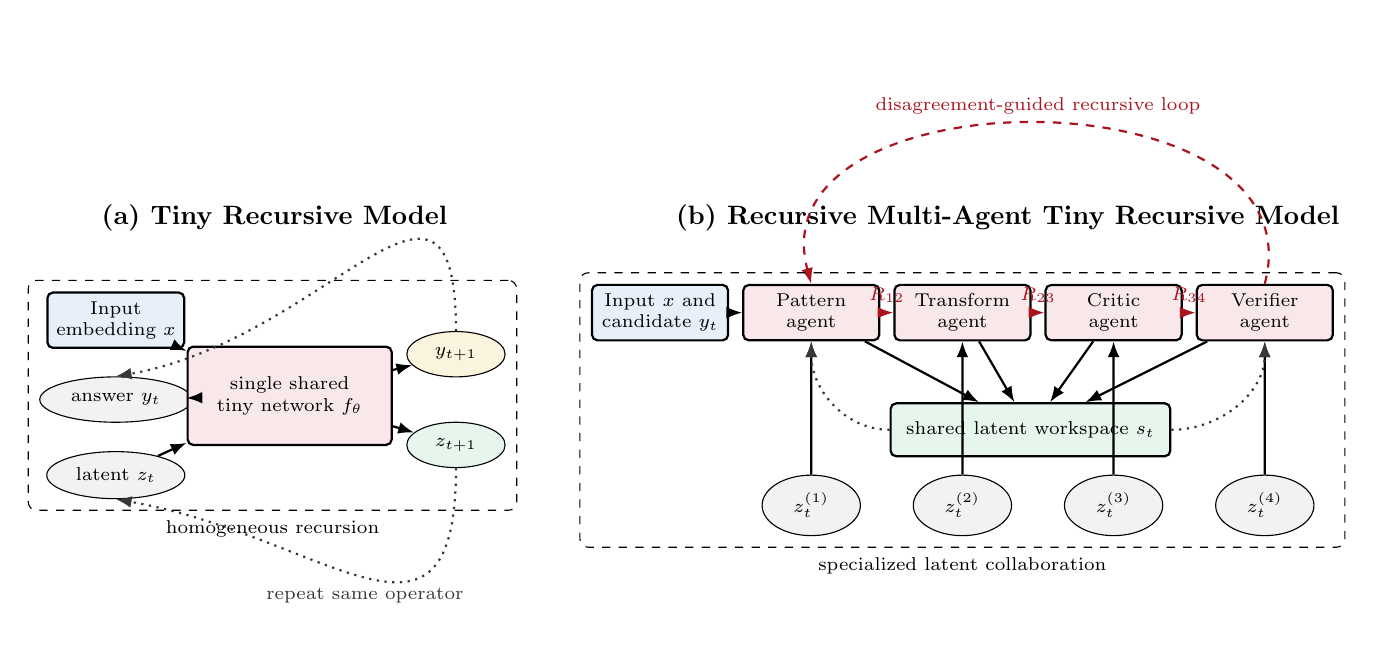
\begin{tikzpicture}[node distance=7mm and 7mm,scale=0.96,transform shape]
% TRM panel
\node[font=\bfseries] at (-5.1,2.25) {(a) Tiny Recursive Model};
\node[block,fill=softblue] (x1) at (-7.2,0.9) {Input\\embedding $x$};
\node[state,fill=softgray] (y1) at (-7.2,-0.15) {answer $y_t$};
\node[state,fill=softgray] (z1) at (-7.2,-1.15) {latent $z_t$};
\node[block,fill=softred,minimum width=27mm,minimum height=13mm] (net1) at (-4.9,-0.1) {single shared\\tiny network $f_\theta$};
\node[state,fill=softgreen] (z2) at (-2.7,-0.75) {$z_{t+1}$};
\node[state,fill=softgold] (y2) at (-2.7,0.45) {$y_{t+1}$};
\draw[arrow] (x1) -- (net1);
\draw[arrow] (y1) -- (net1);
\draw[arrow] (z1) -- (net1);
\draw[arrow] (net1) -- (z2);
\draw[arrow] (net1) -- (y2);
\draw[feedback] (z2.south) to[out=-90,in=-10,looseness=1.6] node[below,font=\scriptsize]{repeat same operator} (z1.south);
\draw[feedback] (y2.north) to[out=90,in=10,looseness=1.6] (y1.north);
\node[group,fit=(x1)(y1)(z1)(net1)(z2)(y2),label={[font=\scriptsize]below:homogeneous recursion}] {};

% MA-TRM panel
\node[font=\bfseries] at (4.6,2.25) {(b) Recursive Multi-Agent Tiny Recursive Model};
\node[block,fill=softblue] (x2) at (0.0,1.0) {Input $x$ and\\candidate $y_t$};
\node[block,fill=softred] (a1) at (2.0,1.0) {Pattern\\agent};
\node[block,fill=softred] (a2) at (4.0,1.0) {Transform\\agent};
\node[block,fill=softred] (a3) at (6.0,1.0) {Critic\\agent};
\node[block,fill=softred] (a4) at (8.0,1.0) {Verifier\\agent};
\node[block,fill=softgreen,minimum width=37mm] (ws) at (4.9,-0.55) {shared latent workspace $s_t$};
\node[state,fill=softgray] (p1) at (2.0,-1.55) {$z_t^{(1)}$};
\node[state,fill=softgray] (p2) at (4.0,-1.55) {$z_t^{(2)}$};
\node[state,fill=softgray] (p3) at (6.0,-1.55) {$z_t^{(3)}$};
\node[state,fill=softgray] (p4) at (8.0,-1.55) {$z_t^{(4)}$};
\draw[arrow] (x2) -- (a1);
\draw[latent] (a1) -- node[above,font=\scriptsize]{$R_{12}$} (a2);
\draw[latent] (a2) -- node[above,font=\scriptsize]{$R_{23}$} (a3);
\draw[latent] (a3) -- node[above,font=\scriptsize]{$R_{34}$} (a4);
\foreach \a/\p in {a1/p1,a2/p2,a3/p3,a4/p4}{\draw[arrow] (\p) -- (\a); \draw[arrow] (\a) -- (ws);}
\draw[feedback] (ws.west) to[out=180,in=-90] (a1.south);
\draw[feedback] (ws.east) to[out=0,in=-90] (a4.south);
\draw[latent] (a4.north) to[out=75,in=105,looseness=1.25] node[above,font=\scriptsize]{disagreement-guided recursive loop} (a1.north);
\node[group,fit=(x2)(a1)(a2)(a3)(a4)(ws)(p1)(p2)(p3)(p4),label={[font=\scriptsize]below:specialized latent collaboration}] {};
\end{tikzpicture}
\caption{Architectural distinction. TRM repeatedly applies one operator to the answer and latent state. \MA{} composes role-specialized updates, preserves private states, communicates through latent links, and maintains a shared workspace.}
\label{fig:trm_vs_matrm}
\end{figure*}

\section{Problem Formulation}
Consider a supervised structured reasoning dataset
\begin{equation}
\mathcal{D}=\{(x^{(n)},y^{\star(n)})\}_{n=1}^{N},
\end{equation}
where $x$ is an input structure and $y^\star\in\{1,\ldots,C\}^{L}$ is a target sequence of $L$ categorical cells. A grid is flattened into $L=H\times W$ cells. The model maintains:
\begin{itemize}
\item input embeddings $X=E_x(x)\in\R^{L\times d}$;
\item an embedded candidate answer $Y_t=E_y(\hat y_t)\in\R^{L\times d}$;
\item $M$ private agent states $Z_t^{(i)}\in\R^{L\times d}$;
\item a shared workspace $S_t\in\R^{L\times d}$;
\item per-agent predictive distributions $P_t^{(i)}\in[0,1]^{L\times C}$.
\end{itemize}
The objective is to learn a recursive system that produces $\hat y_T=y^\star$ with high exact accuracy while minimizing active agents, recursion rounds, parameters, and energy.

\begin{table}[t]
\caption{Principal notation.}
\label{tab:notation}
\centering
\small
\begin{tabular}{ll}
\toprule
Symbol & Meaning \\
\midrule
$M$ & number of specialized agents \\
$T_{\max}$ & maximum collaboration rounds \\
$k_t$ & active agents in round $t$ \\
$Z_t^{(i)}$ & private state of agent $i$ \\
$S_t$ & shared latent workspace \\
$R_{ij}$ & latent link from agent $i$ to $j$ \\
$P_t^{(i)}$ & agent $i$ output distribution \\
$D_t$ & system disagreement score \\
$U_{t,q}$ & uncertainty at cell $q$ \\
$A_t$ & set of active agents \\
$q_t$ & halting probability \\
\bottomrule
\end{tabular}
\end{table}

\section{Recursive Multi-Agent Architecture}
\subsection{Specialized Tiny Agents}
Let the agent set be $\mathcal{A}=\{A_1,\ldots,A_M\}$. In the recommended four-agent design, the roles are pattern discovery, transformation, criticism, and verification. Each agent receives a role embedding $e_i$ and a role-specific adapter while sharing a common tiny backbone $F_\Theta$.

For a backbone layer with hidden input $H$, agent $i$ applies
\begin{align}
\Delta_i(H) &= B_i\,\sigma\!\left(A_i\LN(H)\right), \label{eq:role_adapter}\\
F_i(H) &= F_\Theta(H)+\alpha_i\Delta_i(H), \label{eq:role_conditioned}
\end{align}
where $A_i\in\R^{r_a\times d}$, $B_i\in\R^{d\times r_a}$, $r_a\ll d$, and $\alpha_i$ is a learned scale. The complete input to agent $i$ at round $t$ is
\begin{equation}
H_t^{(i)}=\Psi_i\left(X,Y_t,Z_t^{(i)},S_t,M_t^{(i)},e_i\right), \label{eq:agent_input}
\end{equation}
where $M_t^{(i)}$ is the incoming latent message and $\Psi_i$ is a lightweight fusion operator, implemented by summation after normalization or by a gated projection.

The private state update is
\begin{align}
G_t^{(i)} &= \sigmoid\left(W_g^{(i)}\LN(H_t^{(i)})+b_g^{(i)}\right), \\
\widetilde Z_{t+1}^{(i)} &= F_i(H_t^{(i)}), \\
Z_{t+1}^{(i)} &= G_t^{(i)}\odot\widetilde Z_{t+1}^{(i)}+
\left(1-G_t^{(i)}\right)\odot Z_t^{(i)}. \label{eq:private_update}
\end{align}
The gate reduces destructive overwriting and allows an agent to retain useful role-specific evidence across rounds.

\subsection{Latent Communication}
Decoded communication would require each agent to project hidden states to output classes, make a discrete or soft decision, and re-embed that decision for the next agent. \MA{} instead uses residual low rank latent links:
\begin{equation}
R_{ij}(H)=P_{ij}H+B_{ij}\sigma\!\left(A_{ij}\LN(H)\right), \label{eq:latent_link}
\end{equation}
where $A_{ij}\in\R^{r_\ell\times d_i}$, $B_{ij}\in\R^{d_j\times r_\ell}$, and $P_{ij}$ is the identity when dimensions match. The message to agent $j$ is
\begin{equation}
M_t^{(j)}=R_{ij}\!\left(Z_{t+1}^{(i)}\right). \label{eq:message}
\end{equation}
The residual branch preserves source semantics, and the low rank branch learns role alignment. Unlike text communication, the link remains differentiable and does not pass through an argmax bottleneck.

\subsection{Agent-Specific States and Shared Workspace}
Private states preserve incompatible or complementary hypotheses. A shared workspace integrates evidence needed by all agents. Let the active set at round $t$ be $A_t$. The workspace attention scores are
\begin{align}
e_t^{(i)} &= w_s^\top\tanh\!\left(W_z\Pool(Z_{t+1}^{(i)})+W_s\Pool(S_t)\right),\\
\beta_t^{(i)} &= \frac{\exp(e_t^{(i)})}{\sum_{j\in A_t}\exp(e_t^{(j)})}. \label{eq:workspace_weights}
\end{align}
The integrated proposal is
\begin{equation}
\widetilde S_{t+1}=\sum_{i\in A_t}\beta_t^{(i)}P_iZ_{t+1}^{(i)}, \label{eq:workspace_proposal}
\end{equation}
and the gated workspace update is
\begin{align}
\Gamma_t &= \sigmoid\!\left(W_\gamma[\LN(S_t);\LN(\widetilde S_{t+1})]\right),\\
S_{t+1} &= \Gamma_t\odot S_t+(1-\Gamma_t)\odot\widetilde S_{t+1}. \label{eq:workspace_update}
\end{align}
The answer head receives both the previous candidate and the updated workspace:
\begin{align}
L_{t+1} &= W_o\LN(Y_t+S_{t+1})+b_o,\\
\bar P_{t+1} &= \softmax(L_{t+1}),\\
\hat y_{t+1,q} &= \arg\max_{c}\bar P_{t+1,q,c}. \label{eq:answer_update}
\end{align}

\subsection{Disagreement-Driven Recursion}
Each active agent produces a provisional output distribution
\begin{equation}
P_t^{(i)}=\softmax\!\left(W_o^{(i)}\LN(Z_{t+1}^{(i)}+S_t)\right).
\end{equation}
The weighted mean prediction is
\begin{equation}
\bar P_t=\sum_{i\in A_t}\omega_t^{(i)}P_t^{(i)}, \quad \sum_{i\in A_t}\omega_t^{(i)}=1.
\end{equation}
We define system disagreement by the weighted Jensen-Shannon divergence:
\begin{equation}
D_t=\frac{1}{L}\sum_{q=1}^{L}\sum_{i\in A_t}\omega_t^{(i)}
\KL\!\left(P_{t,q}^{(i)}\,\|\,\bar P_{t,q}\right). \label{eq:disagreement}
\end{equation}
The verifier estimates correctness confidence $C_t\in[0,1]$, while answer change is
\begin{equation}
\Delta_t=\frac{1}{L}\sum_{q=1}^{L}\Ind[\hat y_{t,q}\neq\hat y_{t-1,q}]. \label{eq:answer_change}
\end{equation}
The learned halting probability is
\begin{equation}
q_t=\sigmoid\!\left(w_h^\top[\Pool(S_t);D_t;C_t;\Delta_t;t/T_{\max}]+b_h\right). \label{eq:halting}
\end{equation}
Inference halts when $q_t\ge\tau_h$, $D_t\le\tau_D$, $C_t\ge\tau_C$, and $\Delta_t\le\tau_\Delta$, or when $t=T_{\max}$. This conjunctive rule prevents high confidence alone from terminating an unstable collaboration.

Adaptive computation is related to Adaptive Computation Time \cite{graves2016act}, but the control signal here includes multi-agent disagreement and structured answer stability. The model does not assume convergence to a fixed point. It uses a bounded number of rounds and learns a stopping policy.

\subsection{Sparse Dynamic Routing}
A router activates only a subset of agents:
\begin{align}
r_t &= \softmax\!\left(W_r\Pool([X;Y_t;S_t])+b_r\right),\\
A_t &= \TopK(r_t,k_t). \label{eq:routing}
\end{align}
During training, a straight-through top-$k$ estimator or a Gumbel relaxation can preserve approximate gradients \cite{jang2017gumbel}. The active agent output is weighted by renormalized gate probabilities. Sparse routing follows the general principle of conditional computation and mixture-of-experts models \cite{shazeer2017moe,fedus2021switch}, but routing operates over semantic reasoning roles rather than large feed-forward experts.

To prevent expert collapse, the utilization fraction $u_i$ and mean router probability $v_i$ are regularized:
\begin{equation}
\mathcal{L}_{\mathrm{bal}}=M\sum_{i=1}^{M}u_iv_i. \label{eq:balance_loss}
\end{equation}
A low value is obtained when workload is spread across roles. A separate entropy schedule permits broad exploration early and sharper routing later.

\subsection{Cell-Level Recursive Attention}
Global recursion can repeatedly modify cells that are already correct. For each cell $q$, define predictive uncertainty and disagreement:
\begin{align}
U_{t,q} &= 1-\max_c\bar P_{t,q,c},\\
D_{t,q} &= \sum_{i\in A_t}\omega_t^{(i)}\KL\!\left(P_{t,q}^{(i)}\,\|\,\bar P_{t,q}\right). \label{eq:cell_scores}
\end{align}
A differentiable attention mask is
\begin{equation}
\begin{aligned}
\mu_{t,q}=\sigmoid\!\Big(&\tau^{-1}\big[a_DD_{t,q}+a_UU_{t,q}\\
&+a_\Delta\Ind[\hat y_{t,q}\neq\hat y_{t-1,q}]-\tau_m\big]\Big).
\end{aligned}
\label{eq:cell_mask}
\end{equation}
The next state update is spatially gated:
\begin{equation}
Z_{t+1,q}^{(i)}=\mu_{t,q}\widetilde Z_{t+1,q}^{(i)}+(1-\mu_{t,q})Z_{t,q}^{(i)}. \label{eq:cell_update}
\end{equation}
A periodic global refresh, for example every second round, sets $\mu_{t,q}=1$ for all cells. This prevents early confidence errors from becoming permanently frozen.

\begin{figure}[t]
\centering
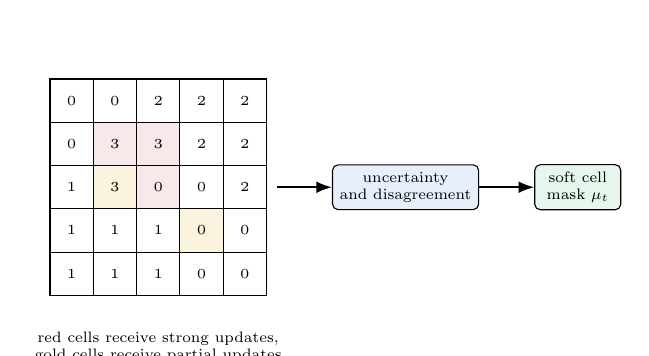
\begin{tikzpicture}[scale=0.78,transform shape]
\matrix[matrix of nodes,nodes={draw,minimum size=5.5mm,font=\tiny,anchor=center},column sep=-\pgflinewidth,row sep=-\pgflinewidth] (g) {
  0 & 0 & 2 & 2 & 2 \\
  0 & |[fill=softred]| 3 & |[fill=softred]| 3 & 2 & 2 \\
  1 & |[fill=softgold]| 3 & |[fill=softred]| 0 & 0 & 2 \\
  1 & 1 & 1 & |[fill=softgold]| 0 & 0 \\
  1 & 1 & 1 & 0 & 0 \\
};
\node[smallblock,fill=softblue,right=9mm of g] (scores) {uncertainty\\and disagreement};
\node[smallblock,fill=softgreen,right=9mm of scores] (mask) {soft cell\\mask $\mu_t$};
\draw[arrow] (g) -- (scores);
\draw[arrow] (scores) -- (mask);
\node[below=3mm of g,font=\scriptsize,align=center] {red cells receive strong updates,\\gold cells receive partial updates};
\end{tikzpicture}
\caption{Cell-level recursive attention. Computation concentrates on unstable output locations while preserving a periodic global refresh.}
\label{fig:cell_attention}
\end{figure}

\section{Collaboration Topologies}
The same agent modules can be connected through four topologies. Let $\Phi_t$ denote one complete collaboration round.

\subsection{Sequential Topology}
Agents form an ordered chain:
\begin{equation}
\Phi_t^{\mathrm{seq}}=A_M\circ R_{M-1,M}\circ A_{M-1}\circ\cdots\circ R_{1,2}\circ A_1. \label{eq:sequential}
\end{equation}
For grid reasoning, a natural sequence is pattern agent, transformation agent, critic, verifier. This topology has low coordination overhead and forms the basis of \MALite.

\subsection{Mixture Topology}
Agents operate in parallel and an integrator combines their states:
\begin{align}
H_t^{(i)} &= A_i(X,Y_t,Z_t^{(i)},S_t),\\
\Phi_t^{\mathrm{mix}} &= A_{\mathrm{int}}\!\left(\sum_{i\in A_t}\beta_t^{(i)}R_{i,\mathrm{int}}(H_t^{(i)})\right). \label{eq:mixture}
\end{align}
This topology is suitable when multiple transformation hypotheses should be explored independently.

\subsection{Deliberation Topology}
A proposer and a critic alternate until the verifier accepts a revised state:
\begin{align}
H_t^{p} &= A_p(S_t),\\
H_t^{c} &= A_c(R_{pc}(H_t^{p}),S_t),\\
H_t^{r} &= A_r(R_{cr}(H_t^{c}),H_t^{p}), \label{eq:deliberation}
\end{align}
where $A_r$ may share the proposer backbone with a revision role adapter. Deliberation allocates more compute to ambiguous tasks but can create oscillation, so the answer-change term in (\ref{eq:halting}) is essential.

\subsection{Distillation Topology}
A stronger collaborative teacher supervises a compact student:
\begin{equation}
\mathcal{L}_{\mathrm{distill}}=T_d^2\KL\!\left(P_T^{(T_d)}\,\|\,P_S^{(T_d)}\right)+\lambda_z\|P_zS_T-Z_S\|_2^2, \label{eq:distill}
\end{equation}
where $T_d$ is the distillation temperature. The student can be a standard TRM or a two-agent \MA. Distillation separates expensive training-time collaboration from low-cost deployment.

\begin{figure*}[t]
\centering
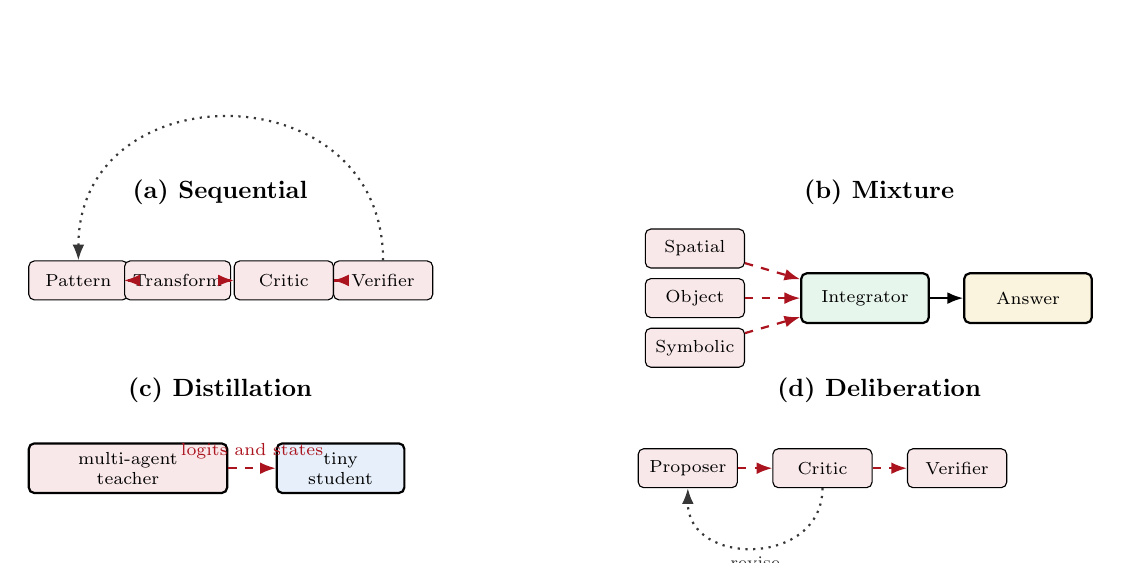
\begin{tikzpicture}[node distance=5mm and 6mm,scale=0.90,transform shape]
% Sequential
\node[font=\bfseries] at (-5.1,2.25) {(a) Sequential};
\node[smallblock,fill=softred] (s1) at (-7.1,1.0) {Pattern};
\node[smallblock,fill=softred] (s2) at (-5.7,1.0) {Transform};
\node[smallblock,fill=softred] (s3) at (-4.2,1.0) {Critic};
\node[smallblock,fill=softred] (s4) at (-2.8,1.0) {Verifier};
\draw[latent] (s1)--(s2);\draw[latent](s2)--(s3);\draw[latent](s3)--(s4);
\draw[feedback] (s4.north) to[out=90,in=90,looseness=1.6] (s1.north);
% Mixture
\node[font=\bfseries] at (4.2,2.25) {(b) Mixture};
\node[smallblock,fill=softred] (m1) at (1.6,1.45) {Spatial};
\node[smallblock,fill=softred] (m2) at (1.6,0.75) {Object};
\node[smallblock,fill=softred] (m3) at (1.6,0.05) {Symbolic};
\node[block,fill=softgreen] (mi) at (4.0,0.75) {Integrator};
\node[block,fill=softgold] (mo) at (6.3,0.75) {Answer};
\draw[latent](m1)--(mi);\draw[latent](m2)--(mi);\draw[latent](m3)--(mi);\draw[arrow](mi)--(mo);
% Distillation
\node[font=\bfseries] at (-5.1,-0.55) {(c) Distillation};
\node[block,fill=softred,minimum width=28mm] (dt) at (-6.4,-1.65) {multi-agent\\teacher};
\node[block,fill=softblue] (ds) at (-3.4,-1.65) {tiny\\student};
\draw[latent] (dt)--node[above,font=\scriptsize]{logits and states}(ds);
% Deliberation
\node[font=\bfseries] at (4.2,-0.55) {(d) Deliberation};
\node[smallblock,fill=softred] (dp) at (1.5,-1.65) {Proposer};
\node[smallblock,fill=softred] (dc) at (3.4,-1.65) {Critic};
\node[smallblock,fill=softred] (dv) at (5.3,-1.65) {Verifier};
\draw[latent](dp)--(dc);\draw[latent](dc)--(dv);
\draw[feedback](dc.south) to[out=-90,in=-90,looseness=1.5] node[below,font=\scriptsize]{revise}(dp.south);
\end{tikzpicture}
\caption{Four collaboration topologies supported by \MA. The topologies use the same latent-link interface and can be compared under matched parameter and computation budgets.}
\label{fig:topologies}
\end{figure*}

\begin{table}[t]
\caption{Properties of the four collaboration topologies.}
\label{tab:topologies}
\centering
\scriptsize
\setlength{\tabcolsep}{3pt}
\begin{tabular}{@{}p{1.35cm}p{3.15cm}p{2.65cm}@{}}
\toprule
Topology & Benefit and principal risk & Suggested use \\
\midrule
Sequential & low overhead and clear roles, but order sensitive & first implementation \\
Mixture & parallel hypotheses, but higher integration cost & ambiguous transformations \\
Deliberation & explicit correction, but possible oscillation & difficult uncertain tasks \\
Distillation & low cost deployment, but teacher bias & compressed inference \\
\bottomrule
\end{tabular}
\end{table}

\section{Inner-Outer Co-Optimization}
\subsection{Inner Role Learning}
The inner stage gives each agent a measurable role competence before full system training. The role losses can be generated from structured corruptions and transformations:
\begin{align}
\mathcal{L}_{\mathrm{pattern}} &= \CE(\hat r,r^\star),\\
\mathcal{L}_{\mathrm{transform}} &= \CE(P^{\mathrm{tr}},y^\star),\\
\mathcal{L}_{\mathrm{critic}} &= \BCE(c,\Ind[\tilde y=y^\star]),\\
\mathcal{L}_{\mathrm{verify}} &= \BCE(v,\Ind[\hat y=y^\star]). \label{eq:role_losses}
\end{align}
Here $r^\star$ denotes an available synthetic relation label, and $\tilde y$ is a corrupted candidate. When explicit relation labels are unavailable, the pattern agent can use contrastive agreement between augmented views.

Let $\theta$ collect shared backbone and adapter parameters, and let $\phi$ collect latent links, router, workspace, attention, and halting parameters. A one-step bilevel form is
\begin{align}
\theta'(\phi) &= \theta-\eta\nabla_\theta\mathcal{L}_{\mathrm{inner}}(\theta,\phi;\mathcal{B}_{\mathrm{in}}), \label{eq:inner_update}\\
\phi &\leftarrow \phi-\beta\nabla_\phi\mathcal{L}_{\mathrm{outer}}(\theta'(\phi),\phi;\mathcal{B}_{\mathrm{out}}). \label{eq:outer_update}
\end{align}
In practice, exact second-order differentiation is optional. A stable implementation alternates several inner updates with one outer update, then performs a final joint fine-tuning stage.

\subsection{Outer System Learning}
The outer stage unrolls the complete system for up to $T_{\max}$ rounds and assigns global credit to all active links and agents. Let $\ell_t=\CE(\bar P_t,y^\star)$. The proposed objective is
\begin{align}
\mathcal{L} ={}& \lambda_f\ell_T
+\lambda_s\sum_{t=1}^{T}w_t\ell_t
+\lambda_{\mathrm{imp}}\mathcal{L}_{\mathrm{imp}}
+\lambda_v\mathcal{L}_{\mathrm{ver}} \nonumber\\
&+\lambda_{\mathrm{spec}}\mathcal{L}_{\mathrm{spec}}
+\lambda_{\mathrm{cons}}\mathcal{L}_{\mathrm{cons}}
+\lambda_{\mathrm{bal}}\mathcal{L}_{\mathrm{bal}} \nonumber\\
&+\lambda_c\mathcal{L}_{\mathrm{compute}}
+\lambda_h\mathcal{L}_{\mathrm{halt}}
+\lambda_m\mathcal{L}_{\mathrm{mask}}. \label{eq:full_loss}
\end{align}
The terms are defined below.

Iterative improvement penalizes rounds that fail to reduce answer loss:
\begin{equation}
\mathcal{L}_{\mathrm{imp}}=\sum_{t=2}^{T}\max(0,\ell_t-\ell_{t-1}+\delta). \label{eq:improvement_loss}
\end{equation}
Verifier calibration uses both correctness and a Brier term:
\begin{equation}
\mathcal{L}_{\mathrm{ver}}=\BCE(C_t,c_t^\star)+\lambda_B(C_t-c_t^\star)^2, \label{eq:verifier_loss}
\end{equation}
where $c_t^\star=\Ind[\hat y_t=y^\star]$ for exact verification, or a normalized cell accuracy target.

Role specialization discourages identical private states:
\begin{equation}
\mathcal{L}_{\mathrm{spec}}=\frac{1}{M(M-1)}\sum_{i\ne j}\left|\cos(\widetilde z^{(i)},\widetilde z^{(j)})\right|, \label{eq:specialization_loss}
\end{equation}
where $\widetilde z^{(i)}$ is a centered pooled state. Output consensus is applied more strongly in later rounds:
\begin{equation}
\mathcal{L}_{\mathrm{cons}}=\sum_{t=1}^{T}\rho_t\sum_{i\in A_t}\omega_t^{(i)}\KL(P_t^{(i)}\|\bar P_t), \quad \rho_{t+1}\ge\rho_t. \label{eq:consensus_loss}
\end{equation}
This schedule permits early hypothesis diversity and late agreement.

Expected computation is regularized by
\begin{equation}
\mathcal{L}_{\mathrm{compute}}=\frac{1}{T_{\max}M}\sum_{t=1}^{T_{\max}}(1-q_{t-1})|A_t|, \label{eq:compute_loss}
\end{equation}
with $q_0=0$. Halting supervision targets the first correct and stable round $t^\dagger$:
\begin{equation}
\mathcal{L}_{\mathrm{halt}}=\sum_{t=1}^{T_{\max}}\BCE(q_t,\Ind[t\ge t^\dagger]). \label{eq:halt_loss}
\end{equation}
The mask sparsity loss is
\begin{equation}
\mathcal{L}_{\mathrm{mask}}=\frac{1}{TL}\sum_{t,q}\mu_{t,q}, \label{eq:mask_loss}
\end{equation}
subject to a minimum update fraction and periodic global refresh.

\begin{algorithm}[t]
\caption{MA-TRM inference with sparse routing and disagreement-driven recursion}
\label{alg:inference}
\small
\begin{algorithmic}[1]
\Require Input $x$, maximum rounds $T_{\max}$, agents $\{A_i\}_{i=1}^{M}$
\State $X\gets E_x(x)$, initialize $\hat y_0$, $Y_0$, $S_0$, $\{Z_0^{(i)}\}$
\For{$t=0$ to $T_{\max}-1$}
  \State $A_t\gets \TopK(\operatorname{Router}(X,Y_t,S_t),k_t)$
  \State compute cell mask $\mu_t$ from uncertainty, disagreement, and change
  \For{each active agent $i$ in topology order}
    \State $M_t^{(i)}\gets R_{j i}(Z_{t+1}^{(j)})$ if predecessor $j$ exists
    \State $\widetilde Z_{t+1}^{(i)}\gets A_i(X,Y_t,Z_t^{(i)},S_t,M_t^{(i)})$
    \State $Z_{t+1}^{(i)}\gets \mu_t\odot\widetilde Z_{t+1}^{(i)}+(1-\mu_t)\odot Z_t^{(i)}$
    \State $P_t^{(i)}\gets \operatorname{Head}_i(Z_{t+1}^{(i)},S_t)$
  \EndFor
  \State $S_{t+1}\gets \operatorname{WorkspaceUpdate}(S_t,\{Z_{t+1}^{(i)}\})$
  \State $(\bar P_{t+1},\hat y_{t+1})\gets \operatorname{AnswerHead}(Y_t,S_{t+1})$
  \State compute $D_{t+1}$, $C_{t+1}$, $\Delta_{t+1}$, and $q_{t+1}$
  \If{$q_{t+1}\ge\tau_h$ and $D_{t+1}\le\tau_D$ and $C_{t+1}\ge\tau_C$ and $\Delta_{t+1}\le\tau_\Delta$}
    \State \textbf{break}
  \EndIf
  \State $Y_{t+1}\gets E_y(\hat y_{t+1})$
\EndFor
\State \Return $\hat y_{t+1}$, diagnostics, and recursion trace
\end{algorithmic}
\end{algorithm}

\begin{algorithm}[t]
\caption{Inner-outer co-optimization}
\label{alg:training}
\small
\begin{algorithmic}[1]
\Require Training data $\mathcal{D}$, inner steps $K$, outer rounds $T_{\max}$
\State initialize shared backbone, role adapters, links, router, workspace, and heads
\For{each training cycle}
  \For{$k=1$ to $K$}
    \State sample $\mathcal{B}_{\mathrm{in}}$ and construct role-specific corruptions
    \State update backbone and role adapters using (\ref{eq:role_losses})
    \State align latent links by state reconstruction or contrastive transfer
  \EndFor
  \State sample $\mathcal{B}_{\mathrm{out}}$
  \State unroll Algorithm~\ref{alg:inference} without hard stopping
  \State compute complete objective in (\ref{eq:full_loss})
  \State update links, router, workspace, attention, halting, and selected adapter parameters
  \State periodically unfreeze the shared backbone for joint low-rate refinement
\EndFor
\State calibrate verifier and halting thresholds on a held-out validation set
\end{algorithmic}
\end{algorithm}

\section{MA-TRM-Lite Recommended Architecture}
\MALite{} is intended as the first reproducible implementation. It uses one shared two-layer backbone, four role adapters, sequential latent collaboration, a shared workspace, top-$k$ routing, a verifier, and at most four collaboration rounds.

\subsection{Agent Roles}
\begin{enumerate}[label=\textbf{A\arabic*.}]
\item \textbf{Pattern agent:} extracts objects, symmetries, repetitions, color relations, and spatial correspondences.
\item \textbf{Transformation agent:} maps detected relations into a candidate output transformation.
\item \textbf{Critic agent:} compares the candidate with demonstrations, detects contradictions, and identifies suspect cells.
\item \textbf{Verifier agent:} estimates exact correctness, cell correctness, and whether another round is beneficial.
\end{enumerate}
The router may skip the critic or pattern agent on simple instances, but the verifier always runs before halting.

\subsection{Round Computation}
For a sequential active path $\pi_t=(i_1,\ldots,i_{k_t})$, one round is
\begin{equation}
H_t^{(i_{j+1})}=A_{i_{j+1}}\!\left(R_{i_j i_{j+1}}(H_t^{(i_j)}),X,Y_t,Z_t^{(i_{j+1})},S_t\right). \label{eq:lite_round}
\end{equation}
After the verifier, the shared workspace and answer are updated. The verifier's state is linked back to the first active agent for the next round.

\begin{figure*}[t]
\centering
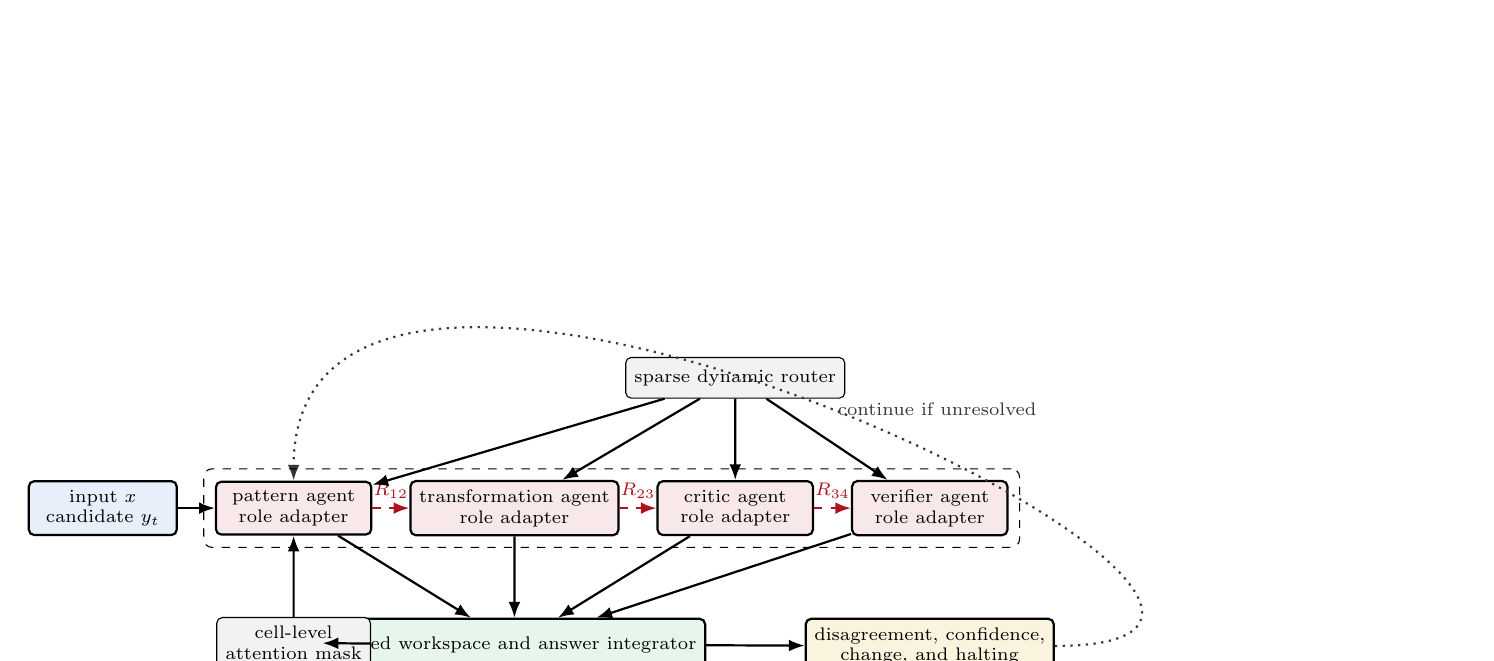
\begin{tikzpicture}[node distance=5mm and 5mm,scale=0.94,transform shape]
\node[block,fill=softblue,minimum width=20mm] (input) {input $x$\\candidate $y_t$};
\node[block,fill=softred,right=of input,minimum width=21mm] (pattern) {pattern agent\\role adapter};
\node[block,fill=softred,right=of pattern,minimum width=21mm] (transform) {transformation agent\\role adapter};
\node[block,fill=softred,right=of transform,minimum width=21mm] (critic) {critic agent\\role adapter};
\node[block,fill=softred,right=of critic,minimum width=21mm] (verify) {verifier agent\\role adapter};
\node[block,fill=softgreen,below=11mm of transform,minimum width=39mm] (workspace) {shared workspace and answer integrator};
\node[block,fill=softgold,below=11mm of verify,minimum width=26mm] (halt) {disagreement, confidence,\\change, and halting};
\node[smallblock,fill=softgray,above=11mm of critic] (router) {sparse dynamic router};
\node[smallblock,fill=softgray,below=11mm of pattern] (mask) {cell-level\\attention mask};
\draw[arrow](input)--(pattern);
\draw[latent](pattern)--node[above,font=\scriptsize]{$R_{12}$}(transform);
\draw[latent](transform)--node[above,font=\scriptsize]{$R_{23}$}(critic);
\draw[latent](critic)--node[above,font=\scriptsize]{$R_{34}$}(verify);
\draw[arrow](pattern)--(workspace);
\draw[arrow](transform)--(workspace);
\draw[arrow](critic)--(workspace);
\draw[arrow](verify)--(workspace);
\draw[arrow](workspace)--(halt);
\draw[feedback](halt.east) to[out=0,in=90,looseness=1.35] node[right,font=\scriptsize]{continue if unresolved}(pattern.north);
\draw[arrow](router)--(pattern);
\draw[arrow](router)--(transform);
\draw[arrow](router)--(critic);
\draw[arrow](router)--(verify);
\draw[arrow](mask)--(pattern);
\draw[arrow](mask)--(workspace);
\node[group,fit=(pattern)(transform)(critic)(verify)] {};
\end{tikzpicture}
\caption{Recommended \MALite{} architecture. Dashed red arrows are continuous latent messages. Solid arrows update the shared workspace. Each role uses a low rank adapter attached to one shared backbone. The router selects active roles, the cell mask controls spatial computation, and the verifier controls recursion.}
\label{fig:lite}
\end{figure*}

\subsection{Default Configuration}
Table~\ref{tab:default_config} gives a conservative starting point. These values are hypotheses for controlled experiments, rather than final tuned values.

\begin{table}[t]
\caption{Recommended initial \MALite{} configuration.}
\label{tab:default_config}
\centering
\small
\begin{tabular}{ll}
\toprule
Component & Initial value \\
\midrule
Shared backbone & 2 layers, width 512 \\
Agents & 4 role-conditioned agents \\
Role adapter rank & $r_a=8$ \\
Latent-link rank & $r_\ell=8$ \\
Maximum rounds & $T_{\max}=4$ \\
Active roles & top 2, verifier mandatory \\
Workspace & gated weighted average \\
Cell mask & soft training, hard inference \\
Precision & bfloat16 where supported \\
Optimization & AdamW with EMA \\
\bottomrule
\end{tabular}
\end{table}

\section{Parameter, Runtime, and Stability Analysis}
\subsection{Controlled Parameter Sharing}
Assume a shared backbone with $P_\Theta$ parameters, $L_b$ adapted layers, hidden width $d$, role adapter rank $r_a$, $M$ agents, $E$ latent links, and link rank $r_\ell$. Ignoring biases and small heads, the total parameter count is
\begin{equation}
P_{\MA}=P_\Theta+2ML_bdr_a+2Edr_\ell+P_{\mathrm{ctrl}}, \label{eq:param_count}
\end{equation}
where $P_{\mathrm{ctrl}}$ includes routing, workspace, verifier, and answer heads.

\begin{proposition}[Parameter overhead]
If $r_a,r_\ell=o(d)$ and $M,E,L_b$ are fixed, then the additional parameters of \MA{} are $o(P_\Theta)$ for a backbone whose dense layers scale as $\Omega(L_bd^2)$.
\end{proposition}
\begin{proof}
The adapter and link overhead in (\ref{eq:param_count}) is $O(L_bMdr_a+Edr_\ell)$. The dense backbone is $\Omega(L_bd^2)$. Their ratio is $O(Mr_a/d+Er_\ell/(L_bd))$, which approaches zero when the ranks grow more slowly than $d$.
\end{proof}

For $d=512$, $L_b=2$, $M=4$, $E=4$, and $r_a=r_\ell=8$, the role adapters and latent links add approximately $98{,}304$ matrix parameters before small control heads. This illustrative calculation indicates that role specialization need not multiply a seven million parameter backbone by four.

Parameter reporting must distinguish the core network, role modules, puzzle identity embeddings, and all other trainable states. This requirement responds directly to concerns that task identity embeddings can materially affect the effective parameter count and generalization interpretation of ARC systems \cite{royeazar2025trmanalysis}.

\subsection{Sparse Compute Bound}
Let one backbone evaluation cost $C_A$, one latent link cost $C_R$, workspace and control cost $C_C$, and let $k_t=|A_t|$.
\begin{proposition}[Sparse round cost]
The cost of an adaptive \MA{} execution is
\begin{equation}
C_{\MA}=\sum_{t=1}^{T}(k_tC_A+(k_t-1)C_R+C_C). \label{eq:runtime}
\end{equation}
Relative to a dense $M$-agent execution with the same number of rounds, the agent-compute ratio is $\sum_t k_t/(TM)$.
\end{proposition}
\begin{proof}
Each active agent incurs one backbone evaluation, each adjacent active pair incurs one link, and each round incurs one control update. Dividing the active agent evaluations by the dense count $TM$ gives the ratio.
\end{proof}

For top-2 routing with four agents, the dominant agent computation is approximately one half of dense four-agent collaboration, before router and verifier overhead. This is a computational accounting statement, not a speed claim. Hardware utilization and kernel launch overhead must be measured.

\subsection{Latent Communication Cost}
Let $C$ be the number of output classes, $d$ the latent width, and $r_\ell$ the link rank. A decoded handoff requires at least an output projection of order $O(LCd)$ and an embedding operation. A low rank latent link costs $O(Ldr_\ell)$, plus an identity residual.

\begin{proposition}[Projection saving]
When agents have equal latent width and $r_\ell<C$, the learned projection component of a low rank latent handoff has lower asymptotic multiplication count than a full class-space decode of the same $L$ positions.
\end{proposition}
\begin{proof}
The link requires two low rank matrix products with order $O(Ldr_\ell)$. The output projection requires order $O(LCd)$. The former is smaller when $r_\ell<C$, up to constant factors.
\end{proof}

For ARC grids, $C$ is small, so raw projection savings alone may be modest. The more important benefits are differentiability, preservation of uncertainty, and avoidance of an argmax bottleneck. The paper therefore treats latent communication as an information and optimization design, rather than claiming universal runtime superiority.

\subsection{Sufficient Stability Condition}
Let $\Phi$ be one complete collaboration-round map on the joint state $\mathcal{S}_t=(S_t,Z_t^{(1)},\ldots,Z_t^{(M)},Y_t)$.

\begin{proposition}[Sufficient contraction condition]
Suppose each active agent and link is Lipschitz continuous, the gated workspace update is nonexpansive, and the product of Lipschitz constants along every active sequential path is at most $\kappa<1$. Then $\Phi$ is a contraction on a closed joint-state domain and repeated rounds converge to a unique fixed state.
\end{proposition}
\begin{proof}
The Lipschitz constant of a composition is at most the product of component constants. Convex gated aggregation is nonexpansive under the stated assumption. Thus $\|\Phi(\mathcal{S})-\Phi(\mathcal{S}')\|\le\kappa\|\mathcal{S}-\mathcal{S}'\|$. The Banach fixed-point theorem gives existence, uniqueness, and convergence.
\end{proof}

This proposition is a diagnostic sufficient condition, not a premise of \MA{} training. The system remains well defined when the condition fails because recursion is explicitly bounded by $T_{\max}$. Spectral normalization or residual scaling may be used if oscillatory trajectories occur.

\subsection{Verifier-Based Error Control}
\begin{assumption}[Cell calibration]
For each cell $q$, the verifier confidence $c_{t,q}$ satisfies $\Pr(\hat y_{t,q}=y_q^\star\mid c_{t,q}=c)=c$ on the validation distribution.
\end{assumption}

\begin{proposition}[Expected Hamming error]
Under cell calibration,
\begin{equation}
\mathbb{E}[d_H(\hat y_t,y^\star)\mid\{c_{t,q}\}]=\sum_{q=1}^{L}(1-c_{t,q}). \label{eq:hamming_bound}
\end{equation}
Therefore, a stopping rule that requires $\sum_q(1-c_{t,q})\le\epsilon$ controls expected Hamming error by $\epsilon$ on the calibration distribution.
\end{proposition}
\begin{proof}
The Hamming error is the sum of cell error indicators. Linearity of expectation and calibration give (\ref{eq:hamming_bound}).
\end{proof}

Disagreement is not itself a correctness certificate because agents can agree on the same wrong answer. It serves as a stability and epistemic diversity signal that complements calibrated verification.

\section{Experimental Methodology}
\subsection{Research Questions}
The evaluation should answer five questions:
\begin{enumerate}[label=\textbf{RQ\arabic*:}]
\item Does role-specialized recursion improve exact accuracy over parameter-matched and compute-matched TRM?
\item Do latent links outperform decoded intermediate handoffs under matched topology and compute?
\item Does disagreement-driven recursion improve accuracy per unit of computation?
\item Do sparse routing and cell-level attention reduce cost without harming exact accuracy?
\item Which collaboration topology provides the best accuracy, calibration, and efficiency trade-off?
\end{enumerate}

\subsection{Benchmarks}
The primary benchmarks are Sudoku-Extreme, Maze-Hard, ARC-AGI-1, and ARC-AGI-2, following the structured reasoning setting established by HRM and TRM \cite{wang2025hrm,jolicoeur2025trm}. Pencil Puzzle Bench may be added to test broader puzzle transfer, particularly because probabilistic TRM reports substantial gains there \cite{sghaier2026ptrm}. ARC tasks should use official splits and carefully documented augmentation.

\subsection{Baselines}
Required baselines include:
\begin{itemize}
\item released TRM configuration;
\item TRM with more recursion rounds;
\item TRM with a parameter increase equal to \MA{} overhead;
\item TRM with matched training and inference FLOPs;
\item HRM where reproducible;
\item probabilistic TRM at matched test-time trajectories;
\item \MA{} without learned links;
\item \MA{} with decoded communication;
\item \MA{} without private states;
\item \MA{} without disagreement-driven halting;
\item dense and sparse \MA{} variants.
\end{itemize}

\subsection{Evaluation Regimes}
To avoid confounding architecture with test-time search, every ARC result should be reported in four regimes:
\begin{enumerate}[label=(\alph*)]
\item canonical single-pass inference;
\item canonical adaptive recursion;
\item augmented inference without voting;
\item augmented multi-sample voting with the exact sample count reported.
\end{enumerate}
Task identity embeddings should be evaluated as an explicit ablation. The main table should report results both with and without identity conditioning. Training data augmentation count, voting count, and total inference FLOPs must appear beside accuracy.

\subsection{Metrics}
The primary quality metric is exact task accuracy. Secondary metrics are cell accuracy, verifier Brier score, expected calibration error, negative log likelihood, and correction rate after the first round. Efficiency metrics are parameter count, active parameter count, FLOPs, peak memory, wall-clock time, GPU-hours, mean rounds, mean active agents, mask density, and energy where measurable. The main combined metric is
\begin{equation}
\mathrm{EfficiencyScore}=\frac{\mathrm{ExactAccuracy}}{\log(1+\mathrm{InferenceFLOPs})}. \label{eq:efficiency_score}
\end{equation}
This score is supplementary. Raw accuracy and raw cost must remain visible.

\subsection{Statistical Protocol}
Use at least five seeds for Sudoku and Maze, and at least three seeds for full ARC experiments. Report mean, standard deviation, and bootstrap confidence intervals for exact accuracy. Compare paired outputs with McNemar's test when systems evaluate the same task set. Hyperparameters must be selected on validation data, and all final evaluation scripts should be frozen before test execution.

\begin{table*}[t]
\caption{Minimum ablation matrix for a publication-quality evaluation. Every row should report exact accuracy, cell accuracy, calibration, parameters, FLOPs, mean rounds, active agents, memory, and GPU-hours.}
\label{tab:ablations}
\centering
\small
\resizebox{\textwidth}{!}{%
\begin{tabular}{p{3.0cm}ccccccp{4.0cm}}
\toprule
Variant & Roles & Latent links & Private states & Disagreement halt & Sparse route & Cell attention & Purpose \\
\midrule
TRM baseline & 1 & no & 1 & no & no & no & reproduce original architecture \\
Parameter-matched TRM & 1 & no & 1 & no & no & no & control for parameter count \\
Compute-matched TRM & 1 & no & 1 & no & no & no & control for recursive compute \\
MA-TRM shared backbone & 4 & yes & yes & no & no & no & isolate specialization \\
MA-TRM decoded messages & 4 & no & yes & no & no & no & compare communication medium \\
MA-TRM no private states & 4 & yes & no & no & no & no & test private memory \\
MA-TRM adaptive & 4 & yes & yes & yes & no & no & test disagreement recursion \\
MA-TRM sparse & 4 & yes & yes & yes & yes & no & test routing efficiency \\
MA-TRM-Lite & 4 & yes & yes & yes & yes & yes & full proposed model \\
\bottomrule
\end{tabular}%
}
\end{table*}

\section{Implementation and Infrastructure}
A faithful implementation can extend the released TRM code structure by adding agents, links, routing, workspace, and control modules. The initial development environment can use a single modern GPU. Full ARC reproduction should follow the original TRM scale, which reports multi-day training on four H100 GPUs in its public repository \cite{trmgithub2026}. Activation checkpointing is recommended because unrolled collaboration stores multiple agent states even when parameter count is small.

The software stack should include Python, PyTorch, CUDA, Distributed Data Parallel, Hydra or an equivalent configuration system, and an experiment tracker. Deterministic and high-performance configurations should be separated. Every run must record the source commit, dataset hash, augmentation policy, random seed, model configuration, driver, CUDA, PyTorch, GPU model, and precision.

The implementation should expose a structured recursion trace containing active agents, router probabilities, per-cell masks, verifier confidence, disagreement, answer changes, and state norms. These traces are necessary to test whether the system performs genuine iterative correction rather than obtaining gains from additional parameters or voting.

\section{Expected Failure Modes and Mitigations}
\subsection{Agent Collapse}
All role adapters may learn nearly identical functions. The specialization loss, role-specific pretraining, router balancing, and representation analysis mitigate this risk. Collapse should be measured by centered kernel alignment and pairwise cosine similarity, rather than inferred from role names.

\subsection{False Consensus}
Agents may agree on an incorrect answer, making disagreement small. Calibrated verification, periodic global refresh, stochastic training corruptions, and optional probabilistic trajectories can provide independent safeguards. Disagreement must never be treated as a correctness certificate.

\subsection{Routing Starvation}
Top-$k$ routing may prevent rarely selected agents from learning. Early training should use higher temperature, occasional random role activation, and a load-balancing objective. The verifier can be mandatory in every round.

\subsection{Oscillatory Deliberation}
The proposer and critic may alternate between incompatible answers. Answer-change penalties, residual damping, maximum-round limits, and spectral control of latent links can reduce oscillation.

\subsection{Mask Lock-In}
Cell attention may freeze an early mistake. Soft masks during training and periodic full-grid refresh prevent irreversible lock-in.

\subsection{Benchmark Leakage and Identity Dependence}
ARC augmentation and task identity embeddings can obscure generalization. The evaluation must disclose exact augmentation procedures, isolate identity features, and report canonical single-pass results \cite{royeazar2025trmanalysis}.

\section{Discussion}
The proposed model treats collaboration as the recursion operator. Standard TRM computes repeated powers of one learned map, approximately $f_\theta^T$. \MA{} computes repeated compositions of role-conditioned maps and latent links:
\begin{equation}
\left(R_{Mi_1}A_M\circ\cdots\circ R_{12}A_1\right)^T. \label{eq:collaborative_operator}
\end{equation}
The design hypothesis is that functional diversity can improve the quality of each recursive step. Controlled sharing prevents this diversity from requiring independent full networks.

Private states and the shared workspace play complementary roles. Private states allow agents to preserve evidence that is temporarily inconsistent with consensus. The shared workspace creates a common answer context and enables system-level credit. Too much consensus early can eliminate useful diversity, while too little consensus late can prevent stable output. The annealed objective in (\ref{eq:consensus_loss}) makes this trade-off explicit.

Disagreement-driven recursion also changes the interpretation of depth. Depth becomes conditional on unresolved evidence rather than a fixed hyperparameter. Sparse routing makes agent count another adaptive axis, and cell attention makes spatial coverage adaptive. Together, the model allocates computation across three dimensions: rounds, roles, and cells.

The strongest version of the research claim should remain modest until experiments are complete. \MA{} is expected to be most useful when tasks benefit from separable operations such as proposal, transformation, criticism, and verification. It may provide little advantage when one homogeneous operator already captures the task or when role supervision causes unnecessary inductive bias.

\section{Limitations}
This paper proposes an architecture and protocol, not a completed empirical study. The mathematical results are conditional accounting and stability statements, not proofs of improved reasoning accuracy. The contraction condition is sufficient but may not hold in trained networks. Verifier error control depends on calibration under the evaluation distribution. Low rank sharing can constrain role diversity too strongly. Sparse routing may reduce hardware efficiency when small irregular kernels dominate. Cell-level masks add control overhead that may exceed their savings on small grids.

The four agent roles are suitable for structured puzzles but may need revision for other domains. Distillation can inherit teacher errors. Deliberation can amplify correlated mistakes. ARC results are particularly sensitive to augmentation, task identity features, and test-time sampling, so claims of general reasoning should be made only after transparent ablations.

\section{Conclusion}
We introduced \MA, a parameter-efficient framework in which tiny specialized reasoners refine a structured solution through latent collaboration. The architecture replaces homogeneous recursion with role-conditioned agents, residual latent links, private states, a shared workspace, disagreement-driven recursion, sparse routing, and cell-level attention. Four collaboration topologies and an inner-outer optimization procedure provide a unified model family. \MALite{} offers a concrete first implementation with a shared two-layer backbone and low rank specialization. The framework yields precise hypotheses about recursive specialization, communication, adaptive computation, and parameter sharing. Its scientific value will depend on parameter-matched, compute-matched, identity-aware, and augmentation-transparent evaluation.

\appendix
\section{Recommended Training Schedule}
A practical curriculum has four stages. Stage one reproduces TRM exactly. Stage two adds role adapters and trains role losses without recursion. Stage three trains latent links and the shared workspace while freezing most backbone parameters. Stage four enables sparse routing, cell attention, and halting, followed by low-rate joint fine-tuning. Suggested loss weights should be tuned by validation, starting with $\lambda_f=1$, $\lambda_s=0.5$, $\lambda_{\mathrm{imp}}=0.1$, $\lambda_v=0.1$, $\lambda_{\mathrm{spec}}=0.01$, $\lambda_{\mathrm{cons}}=0.01$, $\lambda_{\mathrm{bal}}=0.01$, $\lambda_c=10^{-3}$, $\lambda_h=0.05$, and $\lambda_m=10^{-3}$.

\section{Reproducibility Checklist}
A complete release should include source code, environment files, exact dataset construction scripts, trained checkpoints, raw per-task predictions, all configuration files, evaluation scripts, and profiler traces. The paper should report total trainable parameters both with and without task identity embeddings, total forward evaluations, exact test-time sample count, and all stopping thresholds.

\balance
\begin{thebibliography}{99}
\bibitem{chollet2019arc}
F. Chollet, ``On the measure of intelligence,'' arXiv:1911.01547, 2019.

\bibitem{wang2025hrm}
G. Wang, J. Li, Y. Sun, X. Chen, C. Liu, Y. Wu, M. Lu, S. Song, and Y. Abbasi-Yadkori, ``Hierarchical reasoning model,'' arXiv:2506.21734, 2025.

\bibitem{jolicoeur2025trm}
A. Jolicoeur-Martineau, ``Less is more: Recursive reasoning with tiny networks,'' arXiv:2510.04871, 2025.

\bibitem{yang2026recursivemas}
X. Yang, J. Zou, R. Pan, R. Qiu, P. Lu, S. Diao, J. Jiang, H. Tong, T. Zhang, M. J. Buehler, J. He, and J. Zou, ``Recursive multi-agent systems,'' arXiv:2604.25917, 2026.

\bibitem{royeazar2025trmanalysis}
A. Roye-Azar, S. Vargas-Naranjo, D. Ghai, N. Balamurugan, and R. Amir, ``Tiny recursive models on ARC-AGI-1: Inductive biases, identity conditioning, and test-time compute,'' arXiv:2512.11847, revised 2026.

\bibitem{sghaier2026ptrm}
A. Sghaier, A. Parviz, and A. Jolicoeur-Martineau, ``Probabilistic tiny recursive model,'' arXiv:2605.19943, 2026.

\bibitem{graves2016act}
A. Graves, ``Adaptive computation time for recurrent neural networks,'' arXiv:1603.08983, 2016.

\bibitem{fedus2021switch}
W. Fedus, B. Zoph, and N. Shazeer, ``Switch transformers: Scaling to trillion parameter models with simple and efficient sparsity,'' Journal of Machine Learning Research, vol. 23, no. 120, pp. 1--39, 2022.

\bibitem{shazeer2017moe}
N. Shazeer, A. Mirhoseini, K. Maziarz, A. Davis, Q. Le, G. Hinton, and J. Dean, ``Outrageously large neural networks: The sparsely-gated mixture-of-experts layer,'' in Proceedings of the International Conference on Learning Representations, Toulon, France, 2017.

\bibitem{jang2017gumbel}
E. Jang, S. Gu, and B. Poole, ``Categorical reparameterization with Gumbel-Softmax,'' in Proceedings of the International Conference on Learning Representations, Toulon, France, 2017.

\bibitem{hu2021lora}
E. J. Hu, Y. Shen, P. Wallis, Z. Allen-Zhu, Y. Li, S. Wang, L. Wang, and W. Chen, ``LoRA: Low-rank adaptation of large language models,'' in Proceedings of the International Conference on Learning Representations, Virtual, 2022.

\bibitem{vaswani2017attention}
A. Vaswani, N. Shazeer, N. Parmar, J. Uszkoreit, L. Jones, A. N. Gomez, L. Kaiser, and I. Polosukhin, ``Attention is all you need,'' in Advances in Neural Information Processing Systems, Long Beach, CA, pp. 5998--6008, 2017.

\bibitem{bai2019deq}
S. Bai, J. Z. Kolter, and V. Koltun, ``Deep equilibrium models,'' in Advances in Neural Information Processing Systems, Vancouver, Canada, pp. 690--701, 2019.

\bibitem{lee2015deep}
C.-Y. Lee, S. Xie, P. Gallagher, Z. Zhang, and Z. Tu, ``Deeply-supervised nets,'' in Proceedings of the International Conference on Artificial Intelligence and Statistics, San Diego, CA, pp. 562--570, 2015.

\bibitem{franceschi2018bilevel}
L. Franceschi, P. Frasconi, S. Salzo, R. Grazzi, and M. Pontil, ``Bilevel programming for hyperparameter optimization and meta-learning,'' in Proceedings of the International Conference on Machine Learning, Stockholm, Sweden, pp. 1568--1577, 2018.

\bibitem{loshchilov2019adamw}
I. Loshchilov and F. Hutter, ``Decoupled weight decay regularization,'' in Proceedings of the International Conference on Learning Representations, New Orleans, LA, 2019.

\bibitem{polyak1992averaging}
B. T. Polyak and A. B. Juditsky, ``Acceleration of stochastic approximation by averaging,'' SIAM Journal on Control and Optimization, vol. 30, no. 4, pp. 838--855, 1992.

\bibitem{rauba2026tarm}
P. Rauba, C. Fanconi, and M. van der Schaar, ``Tiny autoregressive recursive models,'' arXiv:2603.08082, 2026.

\bibitem{trmgithub2026}
Samsung SAIL Montreal, ``TinyRecursiveModels: Official code for less is more, recursive reasoning with tiny networks,'' GitHub repository, archived Apr. 2026. Available: \url{https://github.com/SamsungSAILMontreal/TinyRecursiveModels}

\bibitem{recursivemasgithub2026}
RecursiveMAS, ``RecursiveMAS: Official implementation for recursive multi-agent systems,'' GitHub repository, 2026. Available: \url{https://github.com/RecursiveMAS/RecursiveMAS}
\end{thebibliography}

\end{document}
